% Declaring packages and formatting
\documentclass[a4paper]{article}

\usepackage{graphicx} % EFor graphics
\usepackage{amsmath} % For mathematics
\usepackage{setspace} % For doublespacing
\usepackage{fancyhdr} % For headers
\usepackage{siunitx} % For SI units
\usepackage[scale=0.75]{geometry} % For wider pages
\usepackage[colorlinks = true, urlcolor = blue, linkcolor = black]{hyperref} % For hyperlinks


% Let's begin the document
\begin{document}
	% Let's set up our headers, footers and doublespacing
	\pagestyle{fancy}
	\renewcommand{\headrulewidth}{0pt}
	\renewcommand{\footrulewidth}{0.4pt}
	\renewcommand{\subsectionmark}[1]{}
	\renewcommand{\sectionmark}[1]{\markboth{#1}{}}
	\cfoot{Last Updated -- \today \\ Tim Snow -- \href{http://www.cunninglemon.com}{http://www.cunninglemon.com} \\ \vspace{1em} 
\includegraphics[height=2em]{Graphics/License}}
	\rfoot{\thepage}
	\doublespacing

	\begin{centering}
 		\section*{Centrifuge Calculator}
 		\label{sec:centrifuge_calculator}
	\end{centering} 	

		\begin{figure}[ht!]
			\centering
			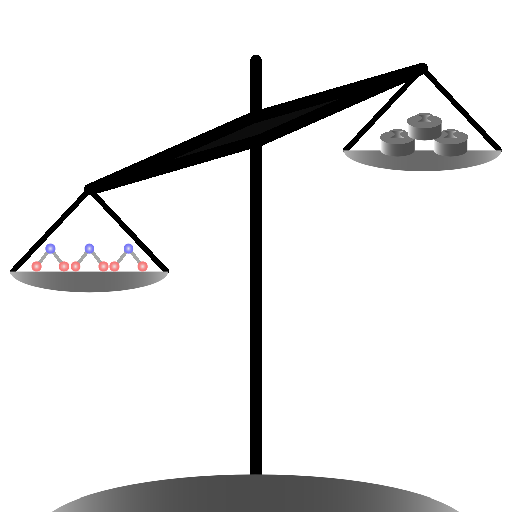
\includegraphics[height=6em]{Graphics/MoleRatioIcon}
		\end{figure}

		\noindent This program has been designed to be small and simple, it will allow the user to calculate the physical masses and molar masses of up to four molecules, related by a ratio, as might be required for a chemical synthesis. It uses the appropriate form of equation \ref{eq:moleEq} to calculate either the molar mass from a physical mass or vice versa. 

		\begin{equation}
			\text{Molar Mass} = \left( \frac{\text{Mass}}{\text{M}_{\text{r}}} \right) \quad \text{or} \quad \text{Mass} = \text{Molar Concentration} \times \text{M}_{\text{r}}
			\label{eq:moleEq}
		\end{equation}

		\noindent The software will detect the molecule you are altering values for and use its relationship to calculate values for the other three molecules, this is dynamic and so will change when the user alters values for a different molecule. Molar masses, and not physical masses, are multiplied by the ratio values with the physical masses being subsequently obtained from their respective molar masses.

		\begin{figure}[ht!]
			\centering
			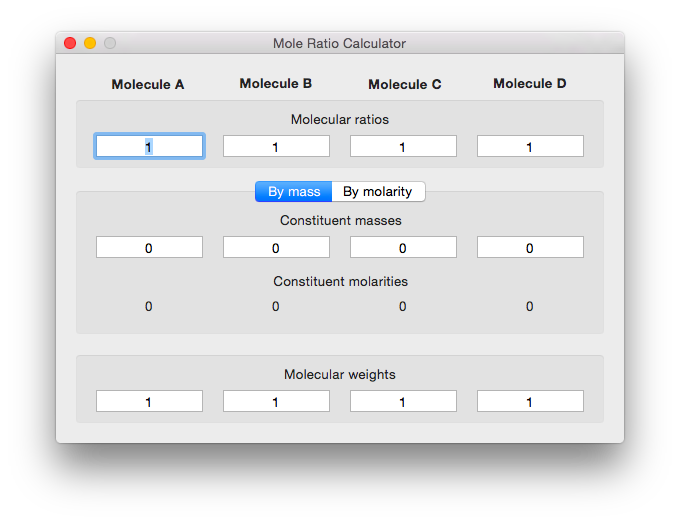
\includegraphics[width=0.4\textwidth]{Graphics/ScreenOne} 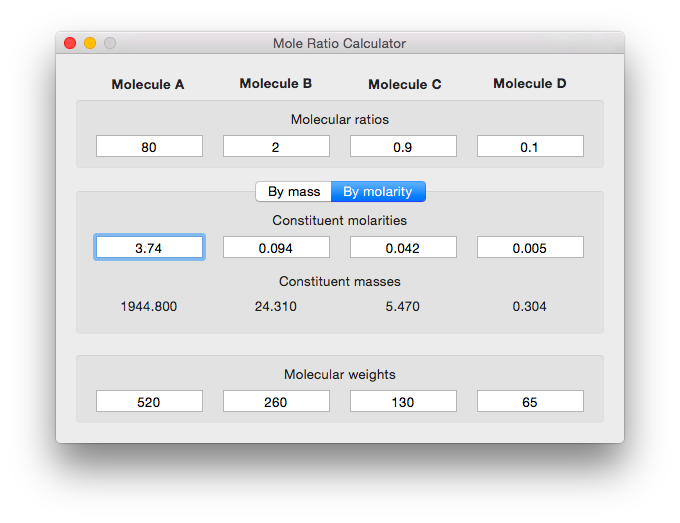
\includegraphics[width=0.4\textwidth]{Graphics/ScreenTwo}
		\end{figure}

		\noindent The figure on the left shows the program startup screen. Simply entering numbers, as shown on the figure on the right, will provide the result requested as both masses and molar concentrations from molar concentrations or masses as input by the user.

		\clearpage


	\begin{centering}
 		\section*{Requirements and License}
 		\label{sec:requirements_and_license}
	\end{centering} 
		
			\noindent This software should work work with any Macintosh computer running Mac OS 10.10 or later and is released under the BSD 3-Clause license, as follows:

			\begin{figure}[ht!]
				\centering
				
\includegraphics[height=6em]{Graphics/BSD}
			\end{figure}

			\begin{quote}
				{\it
					Copyright \textcopyright 2015, Tim Snow\\
					All rights reserved.

					Redistribution and use in source and binary forms, with or without modification, are permitted provided that the following conditions are met:

					1. Redistributions of source code must retain the copyright notice, this list of conditions and the following disclaimer.\\
					2. Redistributions in binary form must reproduce the copyright notice, this list of conditions and the disclaimer found in the license file and/or other materials provided with the distribution.\\
					3. Neither authors' names of its contributors may be used to endorse or promote products derived from this software without specific prior written permission.

					THIS SOFTWARE IS PROVIDED BY THE COPYRIGHT HOLDERS AND CONTRIBUTORS "AS IS" AND ANY EXPRESS OR IMPLIED WARRANTIES, INCLUDING, BUT NOT LIMITED TO, THE IMPLIED WARRANTIES OF MERCHANTABILITY AND FITNESS FOR A PARTICULAR PURPOSE ARE DISCLAIMED. IN NO EVENT SHALL THE COPYRIGHT HOLDER OR CONTRIBUTORS BE LIABLE FOR ANY DIRECT, INDIRECT, INCIDENTAL, SPECIAL, EXEMPLARY, OR CONSEQUENTIAL DAMAGES (INCLUDING, BUT NOT LIMITED TO, PROCUREMENT OF SUBSTITUTE GOODS OR SERVICES; LOSS OF USE, DATA, OR PROFITS; OR BUSINESS INTERRUPTION) HOWEVER CAUSED AND ON ANY THEORY OF LIABILITY, WHETHER IN CONTRACT, STRICT LIABILITY, OR TORT (INCLUDING NEGLIGENCE OR OTHERWISE) ARISING IN ANY WAY OUT OF THE USE OF THIS SOFTWARE, EVEN IF ADVISED OF THE POSSIBILITY OF SUCH DAMAGE.
				}
			\end{quote}
\end{document}